\chapter{Desarrollo del sistema}
\label{cap:capitulo4}

En este capítulo se describe todo el proceso llevado a cabo durante el desarrollo del sistema de detección de emociones y su posterior integración en ROS. Además, se muestran ejemplos de su funcionamiento y se realizan pruebas de rendimiento.

\section{Método de detección de emociones}

Existen múltiples técnicas utilizadas para realizar detección de emociones, en el artículo \cite{literature_review} encontramos una revisión del estado del arte de los últimos años. En este trabajo, se ha escogido la técnica comprendida por los siguientes tres pasos: detección de puntos faciales, extracción de información de esos puntos faciales, clasificación de esa información (Figura \ref{fig:metodo}).\\

\begin{figure} [h!]
  \begin{center}
    \includegraphics[width=16cm]{figs/metodo.png}
  \end{center}
  \captionsetup{justification=centering}
  \caption{Método de detección de emociones.}
  \label{fig:metodo}
\end{figure}

El motivo de esta elección es debido a que es un método con bajo coste computacional y además es de los más precisos, algo esencial para aportar robustez a la herramienta robótica final de este trabajo.

\section{Detección de puntos faciales}

El primer paso del método escogido en este trabajo, consiste en realizar una detección de puntos faciales característicos. En búsqueda de la máxima optimización, se va a hacer un estudio comparando dos librerías de extracción de puntos faciales para obtener conclusiones de cual de ellas nos ofrece más rendimiento y precisión. Las dos librerías son dlib (Sección \ref{sec:dlib}) y MediaPipe (Sección \ref{sec:mediapipe}), escogidas por ser las más usadas dentro de la investigación de este campo en publicaciones como, por ejemplo, los artículos \cite{dlib_emotions} o \cite{mediapipe_emotions}.\\

Las pruebas se realizarán en la Raspberry Pi 4 Model B bajo Raspberry Pi OS, usando la Raspberry Pi Camera como dispositivo para capturar vídeo. Se puede encontrar más información sobre las versiones usadas en el Capítulo \ref{cap:capitulo3}. La resolución utilizada será de 640x480 píxeles y se parte de una media en crudo de 20fps, esto es, sólo mostrando los \textit{frames} (capturados con la librería \textit{picamera}) por pantalla sin ningún tipo de procesamiento.

\subsection{Dlib}

Se comenzará estudiando el rendimiento en FPS ofrecido por dlib y posteriormente se hará un estudio de los fallos producidos por el algoritmo en distintas situaciones. Para realizar las pruebas de rendimiento, se guardará el valor de fps calculado para cada \textit{frame} durante 30 segundos y posteriormente se calculará la media de dichos \textit{frames} guardados. Para realizar las pruebas de fallos, se tendrán en cuenta dos situaciones: falsos positivos y no detección de ningún rostro. Se dará por hecho que siempre hay una cara en cada \textit{frame}, por lo tanto, un \textit{falso positivo} significa que hay más de una cara y \textit{no detección} significa que no hay ninguna. Entonces, se evaluará cada \textit{frame} durante 30 segundos siguiendo esos criterios, y se hará un recuento de los fallos.

\subsubsection{Prueba 1 de rendimiento}

Tal como se ha explicado en la Sección \ref{sec:dlib}, dlib divide la extracción de características faciales en dos pasos: detección del rostro y extracción de características. Para el primero de los pasos, se ofrecen dos opciones incorporadas en sus librerías (HOG y Linear SVM o CNN). En la primera prueba haremos uso del detector de caras basado en HOG y Linear SVM, ya que es el más eficiente computacionalmente hablando, sumado al detector de características también incorporado en las librerías de dlib. Esto ofrece un rendimiento de 0.83 fps de media.

\subsubsection{Prueba 2 de rendimiento}

Tras comprobar el bajo rendimiento obtenido en la primera prueba, se procederá a sustituir el detector de caras usado anteriormente por el detector de caras que trae incorporado OpenCV, este es descrito en el artículo \cite{opencv_haar_cascade}. Se hace uso de este algoritmo porque actualmente es uno de los más rápidos realizando detección facial. Este cambio impulsa el rendimiento de dlib un 656\%, obteniendo una media de 6.28 fps.

\subsubsection{Prueba 3 de rendimiento}
Con el objetivo de mejorar aún más el rendimiento, se procederá a dividir el procesamiento de los \textit{frames} de la lectura de los mismos, haciendo uso de threads. De esta manera se aprovecharán los 4 núcleos del procesador ARM de la Raspberry Pi 4 Model B. Para esto, lo que haremos es lanzar un \textit{thread} que se encargue constantemente de realizar la lectura de los \textit{frames} usando la librería \textit{picamera}, y por otro lado, el thread principal del programa se encargará de realizar el procesamiento de dlib y el detector de caras de OpenCV. Con esto impulsamos el rendimiento un 30\% más, logrando así una media de 8.21 fps. Se puede ver una comparativa de las tres pruebas de rendimiento en la Figura \ref{fig:dlib_rendimiento}.

\begin{figure} [h!]
  \begin{center}
    \includegraphics[width=10cm]{figs/dlib_rendimiento.png}
  \end{center}
  \captionsetup{justification=centering}
  \caption{Comparativa de las tres pruebas de rendimiento de dlib.}
  \label{fig:dlib_rendimiento}
\end{figure}

\subsubsection{Prueba de fallos}

Para comprobar la robustez del algoritmo, se evaluará a este en las siguientes condiciones (Figura \ref{fig:dlib_fallos_ejemplos}):

\begin{itemize}
    \item Buenas condiciones lumínicas: 81 fallos.
    \item Malas condiciones lumínicas: 126 fallos.
    \item Rostros parcialmente cubiertos: 188 fallos.
    \item Rostros girados: 183 fallos.
\end{itemize}

\begin{figure}[h!]
  \begin{center}
    \subcapcentertrue
    \subfigure[Buenas condiciones de luz]{\includegraphics[width=37mm]{figs/dlib_buena_luz.png}}
    \subfigure[Malas condiciones de luz]{\includegraphics[width=37mm]{figs/dlib_mala_luz.png}}
    \subfigure[Rostros cubiertos]{\includegraphics[width=37mm]{figs/dlib_cubiertos.png}}
    \subfigure[Rostros girados]{\includegraphics[width=37mm]{figs/dlib_girados.png}}
  \end{center}
\caption{Condiciones en las que se evalúan los fallos de dlib.}
\label{fig:dlib_fallos_ejemplos}
\end{figure}

\subsection{MediaPipe}
Se comenzará estudiando el rendimiento en FPS ofrecido por MediaPipe y posteriormente se hará un estudio de los fallos producidos por el algoritmo en distintas situaciones. Para realizar las pruebas de rendimiento, se guardará el valor de fps calculado para cada \textit{frame} durante 30 segundos y posteriormente se calculará la media de dichos \textit{frames} guardados. Para realizar la prueba de fallos, a diferencia de dlib, sólo se evaluarán las no detecciones porque los falsos positivos se pueden evitar indicando al algoritmo que sólo detecte una cara. Entonces, se evaluará cada \textit{frame} durante 30 segundos siguiendo esos criterios, y se hará un recuento de los fallos.

\subsubsection{Prueba 1 de rendimiento}
En esta primera prueba se utilizará el algoritmo de la forma general recomendada en el tutorial oficial de MediaPipe. De esta manera, obtenemos una media de 5.91 fps. Este dato es inferior al resultado final de 8.21 fps de dlib.

\subsubsection{Prueba 2 de rendimiento}
Llegados a este punto, para mejorar el resultado anterior, dividimos el procesamiento total en \textit{threads} al igual que hicimos con dlib. Dedicamos un \textit{thread} a la lectura de \textit{frames} y el \textit{thread} principal al procesamiento de MediaPipe. De esta manera, aumentamos el rendimiento un 32\%, obteniendo una media de 7.80fps, todavía sin superar el mejor desempeño de dlib.

\subsubsection{Prueba 3 de rendimiento}
Hasta ahora, estábamos mostrando por pantalla la malla facial detectada, pero esto no será necesario cuando implementemos nuestro sistema de detección de emociones. Por ello, se analizará el rendimiento sin dibujar dicha malla en cada \textit{frame}. De esta manera, el rendimiento sube un 70\% más, llegando así ya a una media de 13.28 fps. Se puede ver una comparativa de las tres pruebas de rendimiento en la Figura \ref{fig:mediapipe_rendimiento}

\begin{figure} [h!]
  \begin{center}
    \includegraphics[width=10cm]{figs/mediapipe_rendimiento.png}
  \end{center}
  \captionsetup{justification=centering}
  \caption{Comparativa de las tres pruebas de rendimiento de MediaPipe.}
  \label{fig:mediapipe_rendimiento}
\end{figure}

\subsubsection{Prueba de fallos}

Para comprobar la robustez del algoritmo, se evaluará a este en las siguientes condiciones (Figura \ref{fig:mediapipe_fallos_ejemplos}):

\begin{itemize}
    \item Buenas condiciones lumínicas: 0 fallos.
    \item Malas condiciones lumínicas: 0 fallos.
    \item Rostros parcialmente cubiertos: 103 fallos.
    \item Rostros girados: 0 fallos.
\end{itemize}

\begin{figure}[h!]
  \begin{center}
  \subcapcentertrue
    \subfigure[Buenas condiciones de luz]{\includegraphics[width=37mm]{figs/mediapipe_buena_luz.png}}
    \subfigure[Malas condiciones de luz]{\includegraphics[width=38mm]{figs/mediapipe_mala_luz.png}}
    \subfigure[Rostros cubiertos]{\includegraphics[width=37mm]{figs/mediapipe_cubiertos.png}}
    \subfigure[Rostros girados]{\includegraphics[width=37mm]{figs/mediapipe_girados.png}}
  \end{center}
\caption{Condiciones en las que se evalúan los fallos de MediaPipe.}
\label{fig:mediapipe_fallos_ejemplos}
\end{figure}

Llegados a este punto, ya habiendo realizado los dos estudios, podemos concluir afirmando que el algoritmo que mejor rendimiento y precisión nos ofrece es el de MediaPipe. Este ha obtenido un rendimiento de 13.28 fps de media, frente a los 8.21 fps de dlib y OpenCV. Además, este último ha obtenido un total de 578 fallos, frente a los 103 fallos de MediaPipe. Por lo tanto, MediaPipe FaceMesh será el algoritmo escogido en este trabajo para obtener la información necesaria de los puntos característicos faciales. Nos brindará información 3D de 468 puntos (Figura \ref{fig:mediapipe_malla}), frente a los 68 que nos hubiera ofrecido dlib.\\

\begin{figure} [h!]
  \begin{center}
    \includegraphics[width=8cm]{figs/canonical_face_model_uv_visualization.png}
  \end{center}
  \captionsetup{justification=centering}
  \caption{Malla facial de MediaPipe de 468 puntos.}
  \label{fig:mediapipe_malla}
\end{figure}

\section{Extracción de información de los puntos faciales}

Tras obtener datos en coordenadas de los puntos faciales característicos de un rostro, debemos tratarlos para que a partir de ellos obtengamos información de las posibles emociones que en ese momento se estén llevando a cabo en el rostro estudiado, y finalmente, crear un dataset con toda esa información que nos permita entrenar modelos de la forma más precisa posible. Esto último es muy importante, porque una de las cosas que determinará la precisión de nuestro modelo, será la existencia de un buen dataset.\\

Retomando la extracción de información, uno de los métodos más usados hasta ahora es la utilización de las distancias entre puntos faciales, tal como se realiza en el artículo \cite{dlib_emotions} (Figura \ref{fig:dlib_foto_articulo}). Por ejemplo, una emoción de \textit{sorpresa} estará caracterizada por poseer grandes distancias entre el labio inferior y la nariz (boca abierta). Sin embargo, esta técnica es propensa a confundir unas emociones con otras, la información de distancias no es suficiente en determinados casos, ya que a veces se puede mantener constante aunque la expresión facial haya cambiado.

\begin{figure} [h!]
  \begin{center}
    \includegraphics[width=7cm]{figs/dlib_foto_articulo.png}
  \end{center}
  \captionsetup{justification=centering}
  \caption{Distancias entre puntos faciales del artículo \cite{dlib_emotions}.}
  \label{fig:dlib_foto_articulo}
\end{figure}

El método usado para extraer información de los puntos faciales, por lo tanto, no será el relatado anteriormente, sino que, se usará un novedoso método propuesto en el artículo \cite{mediapipe_emotions}. Este consiste en construir una \textit{malla emocional} (Figura \ref{fig:malla_emocional}), basada en el Sistema de Codificación Facial o FACS (Facial Action Coding System)\cite{Ekman1978FacialAC}\cite{Ekman1978FacialACManual}, que nos proporcionará información en ángulos de las expresiones faciales.

\begin{figure} [h!]
  \begin{center}
    \includegraphics[width=13cm]{figs/emotional_mesh.png}
  \end{center}
  \captionsetup{justification=centering}
  \caption{\textit{Malla emocional} propuesta en el artículo \cite{mediapipe_emotions}.}
  \label{fig:malla_emocional}
\end{figure}

FACS es un sistema que clasifica movimientos faciales humanos basándose en los cambios producidos en la cara a cargo de los movimientos de los músculos. Estos movimientos son definidos como Unidades de Acción o AUs (Action Units), de los cuales existen hasta 46. En el Cuadro \ref{cuadro:au}, están expuestas las AUs más usadas con sus respectivas descripciones.\\

Además, EMFACS (Emotional Facial Action Coding System) describe emociones simples usando combinaciones de AUs (Cuadro \ref{cuadro:emfacs}). Por lo tanto, sabiendo esto, se puede afirmar que el movimiento de cada uno de esos músculos faciales está relacionado con siete emociones simples, y es por eso, que cada ubicación de los puntos de la \textit{malla emocional} (Figura \ref{fig:malla_emocional}) ha sido elegida de manera que se vea afectada por una AU y de esta manera conseguir un mejor reconocimiento de emociones.\\

\begin{table}[H]
\begin{center}
\begin{tabular}{|c|c|}
     \hline
    \textbf{AU} & \textbf{Descripciones FACS} \\
    \hline
     1 & Interior de las cejas elevado\\ 
     2 & Exterior de las cejas elevado \\ 
     4 & Cejas bajadas \\
     5 & Párpado superior elevado\\
     6 & Mejillas elevadas \\ 
     7 & Párpados tensos \\
     9 & Nariz arrugada \\
     10 & Labio superior elevado \\
     12 & Comisuras de los labios elevados \\ 
     15 & Comisuras de los labios hacia abajo \\
     16 & Labio inferior hacia abajo \\
     17 & Barbilla elevada \\
     20 & Labios apretados y estirados\\
     22 & Labios en forma de \textit{o} \\
     23 & Labios tensos \\
     24 & Labios presionados \\
     25 & Labios separados \\
     26 & Boca abierta (mandíbula caída)\\
     27 & Boca abierta \\
     \hline
 \end{tabular}
 \captionsetup{justification=centering}
\caption{Lista de las Unidades de Acción más usadas y sus respectivas descripciones FACS.}
\label{cuadro:au}
\end{center}
\end{table}

\begin{table}[H]
\begin{center}
\begin{tabular}{|c|c|}
     \hline
    \textbf{Emoción} & \textbf{AU} \\
    \hline
     Felicidad & 6 + 12\\ 
     Tristeza & 1 + 4 + 15 \\ 
     Sorpresa & 1 + 2 + 5 + 26 \\
     Miedo & 1 + 2 + 4 + 5 + 7 + 20 + 26\\
     Enfado & 4 + 5 + 7 + 23 \\ 
     Asco & 9 + 15 + 17 \\
     Desprecio & 12 + 14 \\
     \hline
 \end{tabular}
 \captionsetup{justification=centering}
\caption{Lista de emociones simples en términos de AUs.}
\label{cuadro:emfacs}
\end{center}
\end{table}

Cada uno de los puntos de la \textit{malla emocional} está unido a otros mediante aristas, formando así una malla cerrada de 27 vértices y 38 aristas. Estas aristas forman ángulos entre ellas, y serán estos, los utilizados como información para clasificar emociones. Aprovechando que todas las aristas forman triángulos entre sí (Figura \ref{fig:triangulo}), para calcular los ángulos deseados, se utilizará el teorema del coseno (Ecuación \ref{ec:teorema_coseno}), el cual usa la longitud de las aristas para realizar los cálculos, esto es, la distancia entre los dos puntos que conforman la arista. Esta distancia es calculada mediante distancia euclídea (Ecuación \ref{ec:ecuclidea_puntos}). En forma de código de Python, las funciones que realizarán esta tarea se encuentran en el Código \ref{cod:angulos}.

\begin{figure} [h!]
  \begin{center}
    \includegraphics[width=6cm]{figs/triangulo.png}
  \end{center}
  \captionsetup{justification=centering}
  \caption{Ejemplo de triángulo formado por 2 aristas de la \textit{malla emocional}.}
  \label{fig:triangulo}
\end{figure}

\begin{myequation}[h]
\begin{equation}
\alpha = \arccos{\frac{l_{1}^{2}+l_{3}^{2}-l_{2}^{2}}{2l_{1}l_{3}}}
\nonumber
\label{ec:teorema_coseno}
\end{equation}
\captionsetup{justification=centering}
\caption[Teorema del coseno para calcular el ángulo de la Figura \ref{fig:triangulo}.]{Teorema del coseno para calcular el ángulo de la Figura \ref{fig:triangulo}.}
\end{myequation} 

\begin{myequation}[h]
\begin{equation}
l_{3} = \sqrt{(p_{1x}-p_{2x})^{2}+(p_{1y}-p_{2y})^{2}}
\nonumber
\label{ec:ecuclidea_puntos}
\end{equation}
\captionsetup{justification=centering}
\caption[Distancia euclídea entre los puntos $p_{1}$ y $p_{2}$ de la Figura \ref{fig:triangulo}.]{Distancia euclídea entre los puntos $p_{1}$ y $p_{2}$ de la Figura \ref{fig:triangulo}.}
\end{myequation} 

\begin{code}[h]
\begin{lstlisting}[style=Python]
def distance(self, point1, point2):
    x0 = point1[0]
    y0 = point1[1]
    x1 = point2[0]
    y1 = point2[1]
    return math.sqrt((x0 - x1)**2+(y0 - y1)**2)

def angle(self, point1, point2, point3):
    side1 = self.distance(point2, point3)
    side2 = self.distance(point1, point3)
    side3 = self.distance(point1, point2)
    
    angle = math.degrees(math.acos((side1**2+side3**2-side2**2)/(2*side1*side3)))
    return angle
\end{lstlisting}
\captionsetup{justification=centering}
\caption[Funciones de Python para realizar el cálculo de ángulos\\
de la \textit{malla emocional}.]{Funciones de Python para realizar el cálculo de ángulos\\
de la \textit{malla emocional}.}
\label{cod:angulos}
\end{code}

\section{Generación del dataset}

Siguiendo el esquema de la Figura \ref{fig:metodo}, el paso siguiente a la extracción de información de los puntos faciales es la generación de un dataset (base de datos) con dicha información, para posteriormente entrenar un modelo usando técnicas de Machine Learning, y que este nos permita clasificar emociones. Poseer un buen conjunto de datos es la fase más importante del trabajo, existen proyectos muy buenos que han llegado a fracasar por no poseer un buen dataset. Por lo tanto, hay que dedicar gran parte del tiempo total a la construcción del mismo. Es importante que contenga una buena cantidad de datos y que estos aporten generalidad.\\

La idea a llevar a cabo en este trabajo, es en primer lugar localizar un dataset de imágenes que contenga emociones de distintos sujetos. Seguidamente, tratar cada una de esas imágenes con la \textit{malla emocional} y extraer ángulos de cada una de las emociones. Por último, con esos ángulos se generaría un nuevo dataset, que ya nos serviría para entrenar nuestros modelos. En dicho dataset final, el número de muestras sería el número de fotografías del primer dataset, y el número de características de cada muestra, sería la cantidad de ángulos usados de la \textit{malla emocional}. Un ejemplo de dataset con 224 muestras y cada una de ellas con 21 características se puede encontrar en el Código \ref{cod:ejemplo_dataset}.\\

\begin{code}[h]
\begin{lstlisting}
            X0          X1          X2  ...        X19        X20    y
0    54.288044   37.570711  154.655589  ...  44.625203  63.887010  1.0
1    44.670597   35.229102  148.630240  ...  47.334403  61.278073  1.0
2    46.613914   36.808837  161.148375  ...  57.291823  64.390395  1.0
3    49.404349   47.407905  153.817836  ...  49.880184  61.894869  1.0
4    42.510847   43.626048  146.891826  ...  46.965439  59.971707  1.0
..         ...         ...         ...  ...        ...        ...  ...
220  23.444336   97.667648   88.384186  ...  28.011004  63.905389  7.0
221  24.634940   96.406625   93.413763  ...  28.637606  63.551521  7.0
222  22.425106  105.319774   87.727242  ...  30.811141  61.646881  7.0
223  15.966920  120.968600   60.790043  ...  28.018767  56.442379  7.0
224  19.667632  104.568158   80.332991  ...  29.088510  64.107810  7.0
\end{lstlisting}
\captionsetup{justification=centering}
\caption[Ejemplo de dataset. La primera columna es el número de muestra, \\
la columna \textit{X} son las características, la columna \textit{y} es el tipo de clase.]{Ejemplo de dataset. La primera columna es el número de muestra, \\
la columna \textit{X} son las características, la columna \textit{y} es el tipo de clase.}
\label{cod:ejemplo_dataset}
\end{code}

En cuanto al dataset de imágenes, tras realizar una búsqueda por conseguir las imágenes que mejor se adaptasen a nuestro método, se ha decidido usar \textit{The Extended Cohn-Kanade Dataset (CK+)}\cite{Kanade1}\cite{Kanade2} (Figura \ref{fig:ejemplosCK}). \\

\begin{figure}[h!]
  \begin{center}
    \subcapcentertrue
    \subfigure[Sujeto triste]{\includegraphics[width=50mm]{figs/sujeto_triste.png}}
    \subfigure[Sujeto feliz]{\includegraphics[width=50mm]{figs/sujeto_feliz.png}}
    \subfigure[Sujeto sorprendido]{\includegraphics[width=50mm]{figs/sujeto_sorprendido.png}}
  \end{center}
\captionsetup{justification=centering}
\caption{Ejemplos de imágenes del dataset \textit{The Extended Cohn-Kanade Dataset (CK+)}.}
\label{fig:ejemplosCK}
\end{figure}

Esta base de datos contiene 593 secuencias de imágenes, en las que se muestra un rostro desde una posición neutral hasta la máxima expresión. De esas 593 secuencias, 327 poseen el último \textit{frame} etiquetado con una emoción entre 1 y 7 (1 = anger, 2 = contempt, 3 = disgust, 4 = fear, 5 = happy, 6 = sadness, 7 = surprise). Estos últimos \textit{frames} de esas 327 secuencias, serán los utilizados en este trabajo.\\

CK+ ha sido elegido frente a otro tipo de datasets populares como FER\footnote{FER: \url{https://www.kaggle.com/datasets/msambare/fer2013}}, debido a la alineación de las caras en las imágenes. Bases de datos como la nombrada anteriormente, están enfocadas a ser usadas por CNN (Convolutional Neural Network) y la posición de las caras no influye en el entrenamiento, es más, le aporta más generalidad. Pero para llevar a cabo nuestra técnica, es necesario caras alineadas para obtener información confiable de los ángulos formados por las expresiones faciales. Recordemos que nosostros lo que deseamos es generar un dataset nuevo a partir de otro de imágenes, no utilizar directamente las imágenes como si lo haría una CNN con FER.

\subsection{Cantidad de ángulos a utilizar}

El número de ángulos a utilizar de la \textit{malla emocional}, hará referencia a la cantidad de características que posee nuestro dataset. Es por ello, que se deberá estudiar cuál es la cantidad óptima de los mismos que mejores resultados nos ofrece a la hora de entrenar los modelos.\\

En primer lugar se realizará un estudio para comprobar qué ángulos de toda la malla son más influyentes en las emociones y posteriormente se hará un estudio de simetría con dichos ángulos, para así comprobar si las emociones se pueden considerar simétricas en ambas mitades de un rostro, y de esta manera únicamente utilizar los ángulos de una sola mitad.

\subsubsection{Estudio de influencia}

Tal como se ha comentado anteriormente, realizaremos un estudio para escoger los ángulos más influyentes en cada emoción, esto es, los ángulos que más varían cada vez que se producen dichas expresiones faciales. Para realizar esta prueba, partiremos de todos los ángulos de la parte derecha del rostro (Figura \ref{fig:emotional_mesh_todos_angulos}), y se calculará la variación que existe en cada uno de ellos y para cada una de las emociones de CK+, desde una posición neutral de la cara hasta la máxima expresión.\\

\begin{figure} [h!]
  \begin{center}
    \includegraphics[width=13cm]{figs/emotional_mesh_todos_angulos.png}
  \end{center}
  \captionsetup{justification=centering}
  \caption{Todos los ángulos de la mitad derecha\\
  de la \textit{malla emocional}.}
  \label{fig:emotional_mesh_todos_angulos}
\end{figure}

El método a seguir que nos proporcione esa variación, será calcular la diferencia del ángulo en posición neutral respecto a la posición de la máxima expresión, para ello utilizaremos el Código \ref{cod:angulos_diferencia}. Este, además de calcular la diferencia, evita que aparezcan resultados de otros cuadrantes o negativos. Se realizará este cálculo para cada una de las imágenes de CK+, y los resultados serán las medias calculadas. El resultado del estudio se encuentra en la Figura \ref{fig:estudio_influencia}.\\

\begin{code}[h]
\begin{lstlisting}[language=Python]
def angle_difference(alpha, beta):
    phi = abs(beta-alpha)%360
    if phi > 180:
        return (360 - phi)
    return phi
\end{lstlisting}
\captionsetup{justification=centering}
\caption[Diferencia entre dos ángulos.]{Diferencia entre dos ángulos.}
\label{cod:angulos_diferencia}
\end{code}

Como conclusiones de este estudio, sacamos en claro que los 5 ángulos más influyentes en cada emoción son los mostrados en el Cuadro \ref{cuadro:angulos_5_influyentes}, y que por lo tanto, los ángulos que más varían en total son: 2, 12, 1, 16, 15, 4, 6, 14, 18, 8, 0 y 19.\\

\begin{table}[H]
\begin{center}
\begin{tabular}{|c|c|}
     \hline
    \textbf{Emoción} & \textbf{Ángulos influyentes} \\
    \hline
     Felicidad & 4, 2, 18, 12, 8 \\
     Tristeza & 2, 1, 12, 16, 14 \\
     Sorpresa & 1, 2, 0, 4, 19 \\
     Miedo & 2, 4, 6, 1, 14 \\
     Enfado & 2, 12, 1, 16, 15 \\
     Asco & 12, 16, 2, 15, 1 \\
     Desprecio & 2, 1, 4, 0, 19 \\
     \hline
 \end{tabular}
 \captionsetup{justification=centering}
\caption{Lista de los 5 ángulos más influyentes por cada emoción.}
\label{cuadro:angulos_5_influyentes}
\end{center}
\end{table}

\subsubsection{Estudio de simetría}
Con el afán de descubrir si es posible entrenar a nuestro modelo con sólo ángulos de una mitad del rostro, se va a realizar este estudio de simetría, en el que comprobaremos si las emociones se pueden considerar simétricas para ambos lados de la cara. Para ello, partiremos de los ángulos obtenidos en el estudio anterior (los más influyentes) y generaremos un nuevo mapa que abarque las dos mitades del rostro (Figura \ref{fig:emotional_mesh_2_mitades}).\\

\begin{figure} [h!]
  \begin{center}
    \includegraphics[width=13cm]{figs/emotional_mesh_2_mitades.png}
  \end{center}
  \captionsetup{justification=centering}
  \caption{Mapa de ángulos para realizar el estudio de simetría.}
  \label{fig:emotional_mesh_2_mitades}
\end{figure}

A la hora de estudiar la simetría, calcularemos la variación que existe entre los ángulos del lado izquierdo y del lado derecho, para cada una de las emociones y cada una de las imágenes del dataset CK+. La forma de llevar a cabo este cálculo, será la misma que en el estudio anterior (Código \ref{cod:angulos_diferencia}). Los resultados serán la media de lo obtenido para todas las imágenes, estos se encuentran en la Figura \ref{fig:estudio_simetría}.\\

Finalmente, observando los resultados, podemos considerar que las emociones son simétricas, ya que la mayor variación de media entre el lado izquierdo y derecho ha sido de 5 grados, siendo esta una variación mínima.

\subsubsection{Conclusiones}

Recapitulando, una vez realizados los dos estudios, se procederá ya a generar los dataset. Crearemos dos bases de datos:

\begin{itemize}
    \item Base de datos con todos los ángulos de la parte derecha de la \textit{malla emocional}.
    \item Base de datos con sólo los ángulos más influyentes de la parte derecha de la \textit{malla emocional}.
\end{itemize}

Estos se generan en un fichero csv, en el que cada fila será una muestra, esto es, los datos obtenidos de una imagen de CK+, por lo tanto, poseerá tantas filas como imágenes procesadas. Y cada una de esas filas, tendrá tantas columnas como ángulos calculados en la imagen, y además, una última columna que indicará que tipo de emoción es.
En la siguiente sección se analizará cual de las dos bases de datos nos ofrece mejor rendimiento en el entrenamiento.

\section{Entrenamiento del modelo}
\label{sec:entrenamiento}

Se va a realizar el entrenamiento con tres algoritmos de clasificación diferentes y se compararan los resultados de cada uno de ellos. Los algoritmos a utilizar serán KNN, SVM y MLP. Además, se hará uso de PCA para mejorar la precisión de la detección de emociones. Se estudiará si ofrece mejor resultado el dataset con ángulos reducidos o el que posee todos los ángulos, pero reduciendo estos a través de PCA.\\

Cada uno de los algoritmos posee unos parámetros a optimizar en la fase de entrenamiento, nuestro labor será encontrar aquellos valores que proporcionen más precisión al modelo sin llegar a sobreentrenarlo. En caso de KNN se deberá encontrar el número de vecinos óptimo (k), para SVM el parámetro de regulación óptimo (C) y para MLP el número de capas ocultas y neuronas óptimas. Los demás parámetros de configuración como la función de activación en MLP o el algoritmo para calcular distancias en KNN, se dejarán por defecto tal como los ofrece Scikit-Learn, son los que mejores resultados ofrecen.\\

A la hora de conocer la precisión obtenida durante el entrenamiento, existen varios valores que puntúan el desempeño del modelo:

\begin{itemize}
    \item \textit{Precision.} De las predicciones que ha realizado, indica que porcentaje son correctas.
    \item \textit{Recall.} De los datos, indica que porcentaje están bien predichos.
    \item \textit{F1-Score.} Hace referencia a la media ponderada entre \textit{Precision} y \textit{Recall}.
    \item \textit{Accuracy.} La suma de los aciertos entre el número total de muestras, osea el porcentaje de acierto.
\end{itemize}

Y por último, para evitar el sobreentrenamiento y generalizar los modelos, se hará uso de la validación cruzada K-Fold. Este método nos permitirá usar todos los datos como test y todos los datos como entrenamiento. Esto se consigue gracias a que el algoritmo divide el conjunto de datos en \textit{K pliegues}, y uno de ellos es dedicado a datos de test. Entonces, por cada iteración este conjunto de test se va desplazando a la derecha. En la Figura \ref{fig:kfolf_explicacion}, encontramos un ejemplo de 4 \textit{pliegues}.\\

\begin{figure} [h!]
  \begin{center}
    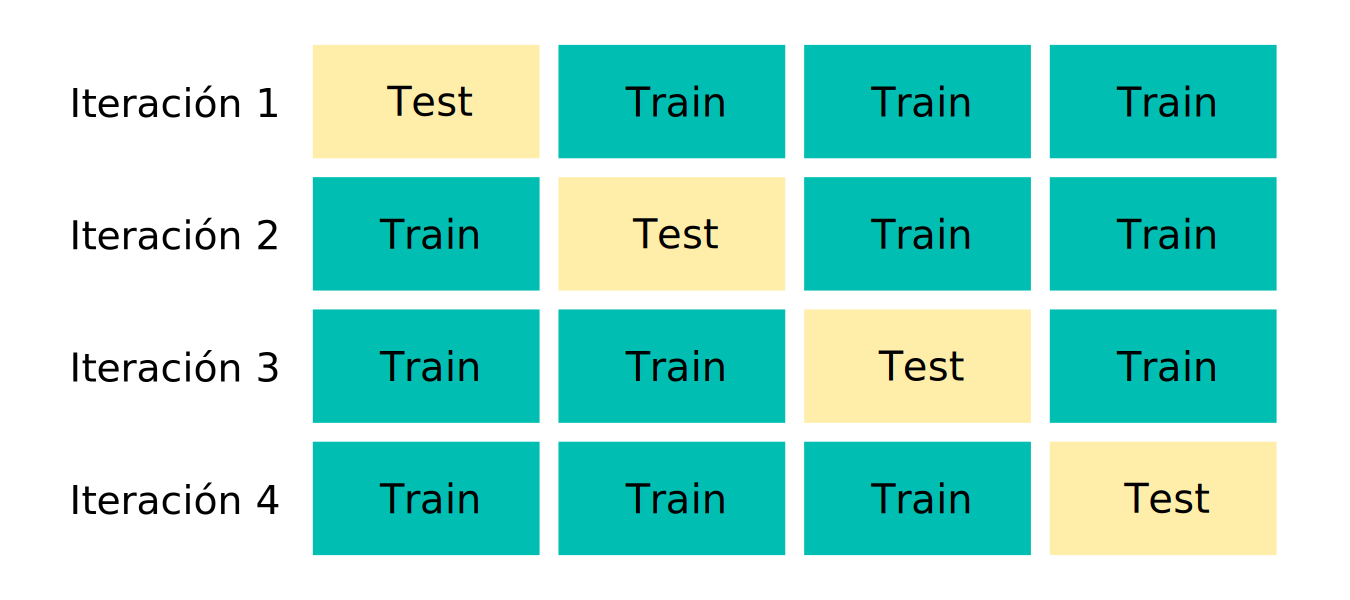
\includegraphics[width=10cm]{figs/KFold_explanation.png}
  \end{center}
  \captionsetup{justification=centering}
  \caption{Ejemplo de división de la base de datos \\
  en 4 \textit{pliegues} usando KFold.}
  \label{fig:kfolf_explicacion}
\end{figure}

La clase con menos datos del dataset CK+, tiene una cantidad de 28. Por lo tanto, se usarán 4 \textit{pliegues} para KFold, de esta manera aseguramos 8 datos de esa clase en cada pliegue. Al tener una base de datos desequilibrada, esto es, que no tiene el mismo número de muestras para todas las clases, debemos usar KFoldStratified, que nos asegura poseer siempre el mismo porcentaje de muestras de cada clase en todos los pliegues.\\

KFoldStratified por lo tanto, nos servirá para encontrar los parámetros óptimos de cada algoritmo. Por ejemplo, para KNN probaremos cada una de las \textit{k} (vecinos) posibles en cada una de las iteraciones. El resultado sería una matriz con el \textit{Accuracy} para cada una de las \textit{k} en cada una de las iteraciones. Finalmente, se calcularía la media de todas las iteraciones y escogeríamos la \textit{k} que más \textit{Accuracy} de media haya obtenido. Esto sería el número de vecinos óptimo. Un ejemplo con 4 valores de vecinos se muestra en la Figura \ref{fig:kfold_KNN}.\\

\begin{figure} [h!]
  \begin{center}
    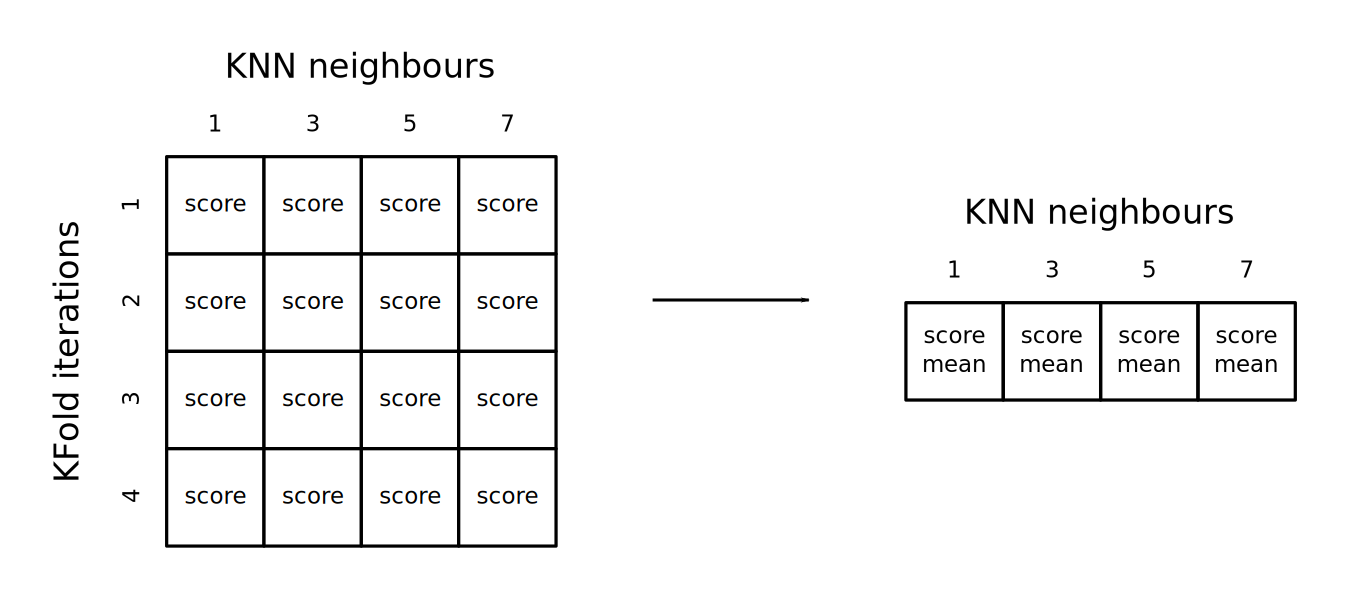
\includegraphics[width=13cm]{figs/KFold_KNN.png}
  \end{center}
  \captionsetup{justification=centering}
  \caption{Ejemplo de búsqueda del número de vecinos\\
  óptimo para KNN usando KFold.}
  \label{fig:kfold_KNN}
\end{figure}

Para el caso en el que además usemos PCA para reducir el número de características (componentes), debemos encontrar además el número óptimo de las mismas. Entonces, en vez de tener una matriz de 2 dimensiones, pasamos a trabajar con una matriz de 3 dimensiones. Se puede ver un ejemplo en la Figura \ref{fig:kfold_KNN_PCA}. Al igual que en el caso anterior, la combinación óptima de vecinos y componentes de PCA, será la que haya obtenido mejor puntuación de media.\\

\begin{figure} [h!]
  \begin{center}
    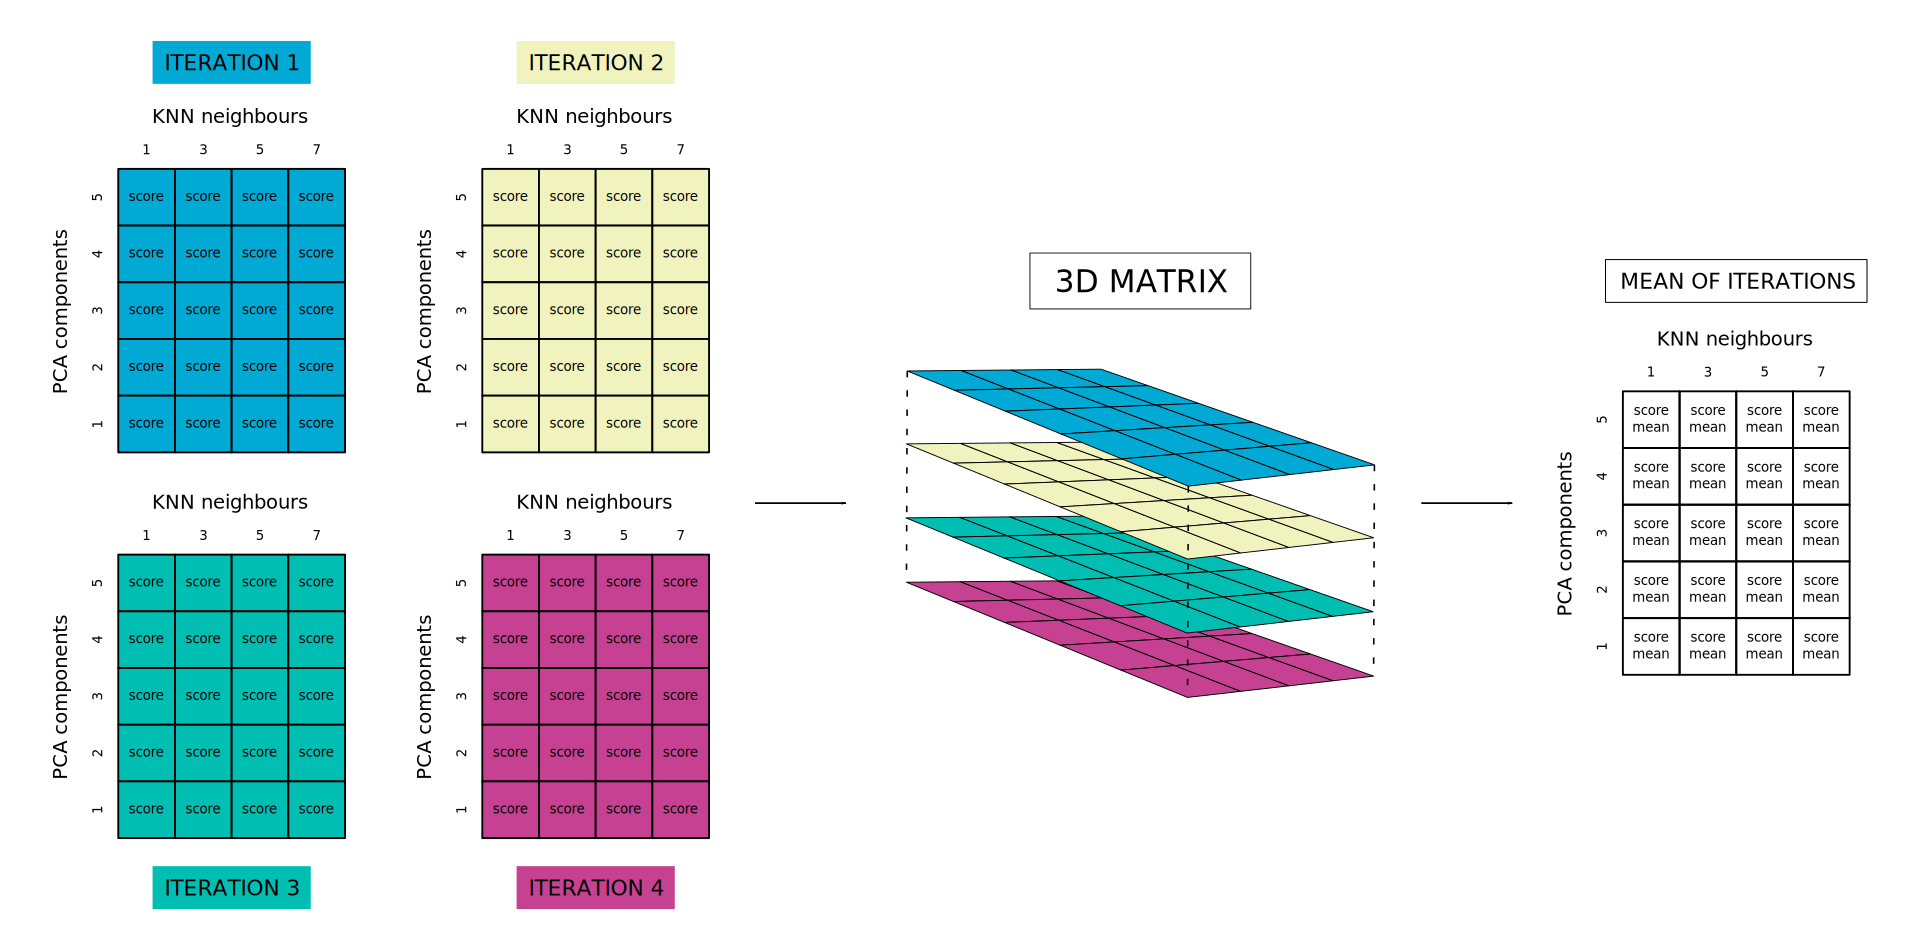
\includegraphics[width=16cm]{figs/KFold_KNN_PCA.png}
  \end{center}
  \captionsetup{justification=centering}
  \caption{Ejemplo de búsqueda del número de vecinos\\
  óptimo para KNN y el número de componentes\\
  óptimo a reducir por PCA usando KFold.}
  \label{fig:kfold_KNN_PCA}
\end{figure}

\subsection{Dataset de ángulos influyentes}

Los parámetros óptimos, para el dataset de ángulos influyentes, tras realizar su búsqueda usando validación cruzada KFoldStratified de 4 \textit{pliegues}, se encuentran en el Cuadro \ref{cuadro:parametros_dataset1}. Para KNN se ha probado con valores de k impares entre 1 y 13 incluidos, para SVM con valores de C entre 1 y 999 (saltos de 10 en 10) y para MLP se ha probado con 1 capa oculta de neuronas entre 5 y 24 incluidos, no ha sido necesario añadir más capas.\\

\begin{table}[H]
\begin{center}
\begin{tabular}{|c|c|}
     \hline
    \textbf{Clasificador} & \textbf{Parámetros} \\
    \hline
     KNN & \verb|k = 11| \\
     SVM & \verb|C = 11| \\
     MLP & \verb|hidden_layer_sizes = (19)|\\
     \hline
 \end{tabular}
 \captionsetup{justification=centering}
\caption{Parámetros óptimos para cada uno de los clasificadores\\
entrenando el dataset de ángulos influyentes.}
\label{cuadro:parametros_dataset1}
\end{center}
\end{table}

Finalmente, los resultados obtenidos en el entrenamiento para dicho dataset y los parámetros, se encuentran en el Cuadro \ref{cuadro:resultados_dataset1}. Estos han sido calculados también mediante validación cruzada KFoldStratified de 4 \textit{pliegues}, y se muestra la media de todas las iteraciones.\\

\begin{table}[H]
\begin{center}
\begin{tabular}{|c|c|c|c|c|}
     \hline
    \textbf{Clasificador} & \textbf{Accuracy} & \textbf{Precision} & \textbf{Recall} & \textbf{F1-score}\\
    \hline
     KNN & 0.82 & 0.76 & 0.74 & 0.74\\
     SVM & 0.84 & 0.79 & 0.78 & 0.77\\
     MLP & 0.82 & 0.78 & 0.78 & 0.77\\
     \hline
 \end{tabular}
 \captionsetup{justification=centering}
\caption{Resultados de precisión de los clasificadores con\\
el dataset de ángulos influyentes.}
\label{cuadro:resultados_dataset1}
\end{center}
\end{table}

\subsection{Dataset de todos los ángulos}

Tal como se ha comentado en la Sección \ref{sec:entrenamiento}, como este dataset posee todos los ángulos de una mitad del rostro, se usará PCA para hacer la reducción de características (ángulos). El valor óptimo de características a reducir y los parámetros para cada clasificador, tras realizar su búsqueda usando validación cruzada KFoldStratified de 4 \textit{pliegues}, se encuentran en el Cuadro \ref{cuadro:parametros_dataset2}. Para hacer la reducción con PCA, se ha probado con un número de componentes entre 2 y 20 incluidos, para KNN se ha probado con valores de k impares entre 1 y 13 incluidos, para SVM con valores de C entre 1 y 999 (saltos de 10 en 10) y para MLP se ha probado con 1 capa oculta de neuronas entre 5 y 24 incluidos, no ha sido necesario añadir más capas.\\

\begin{table}[H]
\begin{center}
\begin{tabular}{|c|c|}
     \hline
    \textbf{Clasificador y PCA} & \textbf{Parámetros} \\
    \hline
     KNN y PCA & \verb|k = 11|, \verb|n_components = 17|\\
     SVM y PCA & \verb|C = 11|, \verb|n_components = 7|\\
     MLP y PCA & \verb|hidden_layer_sizes = (12)|, \verb|n_components = 11|\\
     \hline
 \end{tabular}
 \captionsetup{justification=centering}
\caption{Parámetros óptimos para cada uno de los clasificadores\\
entrenando el dataset de todos los ángulos.}
\label{cuadro:parametros_dataset2}
\end{center}
\end{table}

Finalmente, los resultados obtenidos en el entrenamiento para dicho dataset (reduciendo el número de características con PCA) y los parámetros óptimos, se encuentran en el Cuadro \ref{cuadro:resultados_dataset2}. Estos resultados de precisión han sido calculados también mediante validación cruzada KFoldStratified de 4 \textit{pliegues}, y se muestra la media de todas las iteraciones.\\

\begin{table}[H]
\begin{center}
\begin{tabular}{|c|c|c|c|c|}
     \hline
    \textbf{Clasificador} & \textbf{Accuracy} & \textbf{Precision} & \textbf{Recall} & \textbf{F1-score}\\
    \hline
     KNN & 0.83 & 0.79 & 0.75 & 0.75\\
     SVM & 0.84 & 0.80 & 0.77 & 0.78\\
     MLP & 0.84 & 0.81 & 0.80 & 0.80\\
     \hline
 \end{tabular}
 \captionsetup{justification=centering}
\caption{Resultados de precisión de los clasificadores con\\
el dataset de todos los ángulos, reducido con PCA.}
\label{cuadro:resultados_dataset2}
\end{center}
\end{table}

\subsection{Conclusiones y propuesta de mejora}
Los resultados obtenidos para cada uno de los datasets son bastante similares, aunque un poco superiores para el dataset de todos los ángulos con reducción de características usando PCA, sobre todo si observamos \textit{Precision}, \textit{Recall} y \textit{F1-score}. En cuanto a los resultados obtenidos por cada clasificador, también son muy similares y sería muy complicado decantarse por uno sólo.\\

Sin embargo, en general no son resultados demasiado buenos y la herramienta robótica construida a partir de estos modelos no sería muy robusta. Sobre todo si observamos los resultados de cada una de las clases por separado, por ejemplo los arrojados por SVM usando el dataset de todos los ángulos (Cuadro \ref{cuadro:resultados_SVM}). En dichos resultados, podemos observar que clases como ---por ejemplo--- la de \textit{Desprecio} o la de \textit{Enfado} han obtenido puntuaciones realmente malas, incluso por debajo del 50\% en algún caso. Por lo tanto, esto nos lleva a pensar que nuestro sistema no va a dar buen rendimiento a la hora de detectar todas las emociones, aunque de media si que tenga una puntuación aceptable.\\

\begin{table}
\begin{minipage}{0.48\linewidth}
\centering
\begin{adjustbox}{max width=\textwidth}
\begin{tabular}{|c|c|c|c|}
\hline
\textbf{Clase} & \textbf{Precision} & \textbf{Recall} & \textbf{F1-score}\\
\hline
     Enfado & 0.67 & 0.50 & 0.57\\
     Desprecio & 0.67 & 0.50 & 0.57\\
     Asco & 0.76 & 0.87 & 0.81\\
     Miedo & 0.67 & 1.00 & 0.80\\
     Felicidad & 0.94 & 0.94 & 0.94\\
     Tristeza & 0.83 & 0.71 & 0.77\\
     Sorpresa & 0.95 & 0.95 & 0.95\\
\hline
\end{tabular}
\end{adjustbox}
\vspace{0.5cm}

\begin{adjustbox}{max width=\textwidth}
\begin{tabular}{|c|c|c|c|}
\hline
\textbf{Clase} & \textbf{Precision} & \textbf{Recall} & \textbf{F1-score}\\
\hline
     Enfado & 0.75 & 0.82 & 0.78\\
     Desprecio & 0.67 & 0.80 & 0.73\\
     Asco & 0.82 & 0.93 & 0.87\\
     Miedo & 0.80 & 0.67 & 0.73\\
     Felicidad & 0.94 & 0.94 & 0.94\\
     Tristeza & 1.00 & 0.57 & 0.73\\
     Sorpresa & 0.95 & 0.95 & 0.95\\
\hline
\end{tabular}
\end{adjustbox}
\end{minipage}\hfill
\begin{minipage}{0.48\linewidth}
\centering
\begin{adjustbox}{max width=\textwidth}
\begin{tabular}{|c|c|c|c|}
\hline
\textbf{Clase} & \textbf{Precision} & \textbf{Recall} & \textbf{F1-score}\\
\hline
     Enfado & 0.71 & 0.45 & 0.56\\
     Desprecio & 0.57 & 0.80 & 0.67\\
     Asco & 0.76 & 0.93 & 0.84\\
     Miedo & 1.00 & 0.71 & 0.83\\
     Felicidad & 0.85 & 1.00 & 0.92\\
     Tristeza & 0.83 & 0.71 & 0.77\\
     Sorpresa & 1.00 & 0.95 & 0.98\\
\hline
\end{tabular}
\end{adjustbox}
\vspace{0.5cm}

\begin{adjustbox}{max width=\textwidth}
\begin{tabular}{|c|c|c|c|}
\hline
\textbf{Clase} & \textbf{Precision} & \textbf{Recall} & \textbf{F1-score}\\
\hline
     Enfado & 0.67 & 0.55 & 0.60\\
     Desprecio & 0.50 & 0.25 & 0.33\\
     Asco & 0.67 & 0.80 & 0.73\\
     Miedo & 1.00 & 0.67 & 0.80\\
     Felicidad & 1.00 & 1.00 & 1.00\\
     Tristeza & 0.50 & 0.71 & 0.59\\
     Sorpresa & 1.00 & 1.00 & 1.00\\
\hline
\end{tabular}
\end{adjustbox}
\end{minipage}
\captionsetup{justification=centering}
\caption{Resultados del entrenamiento con SVM en cada una\\
de las 4 iteraciones de KFoldStratified, usando el dataset\\
de todos los ángulos.}
\label{cuadro:resultados_SVM}
\end{table}

Esta mala clasificación de algunas emociones, se debe a la gran similitud que existe entre varias. Esto provoca que geométricamente sean prácticamente indiferenciables, y por lo tanto, es complicado que los algoritmos sepan clasificarlas correctamente. Si observamos el estudio de ángulos influyentes en cada emoción (Figura \ref{fig:estudio_influencia}), podemos ver que ---por ejemplo--- las emociones \textit{sorpresa} y \textit{desprecio} poseen exactamente los mismos 5 ángulos influyentes, o las emociones \textit{enfado} y \textit{asco} que también poseen los mismos 5 (Cuadro \ref{cuadro:angulos_5_influyentes}). Esto dificulta muchísimo la tarea de clasificación.\\

Por lo tanto, se propone eliminar las emociones que estén interceptando con otras, y de esta manera, aumentar la robustez de nuestra futura herramienta, consiguiendo mayor precisión en nuestro modelo. Las emociones que se elegirán, son las siguientes: \textit{felicidad}, \textit{tristeza}, \textit{sorpresa} y \textit{enfado}. Son las 4 emociones simples más generales, y además, se diferencian geométricamente unas de otras.\\

Se usará el dataset con todos los ángulos (reducido con PCA), ya que es con el que se ha obtenido una precisión ligeramente superior, pero esta vez únicamente con las clases: \textit{felicidad}, \textit{tristeza}, \textit{sorpresa} y \textit{enfado}. Utilizando la técnica de validación cruzada, de la misma manera que en las secciones anteriores, los parámetros óptimos encontrados para cada uno de los algoritmos se encuentran en el Cuadro \ref{cuadro:parametros_dataset3}. Y los resultados del entrenamiento con dichos parámetros óptimos, en el Cuadro \ref{cuadro:resultados_dataset3}.\\

\begin{table}[H]
\begin{center}
\begin{tabular}{|c|c|}
     \hline
    \textbf{Clasificador y PCA} & \textbf{Parámetros} \\
    \hline
     KNN y PCA & \verb|k = 7|, \verb|n_components = 11|\\
     SVM y PCA & \verb|C = 21|, \verb|n_components = 11|\\
     MLP y PCA & \verb|hidden_layer_sizes = (17)|, \verb|n_components = 11|\\
     \hline
 \end{tabular}
 \captionsetup{justification=centering}
\caption{Parámetros óptimos para cada uno de los clasificadores\\
entrenando con el dataset de todos los ángulos (\textit{felicidad}, \\
\textit{tristeza}, \textit{sorpresa} y \textit{enfado}), reducido con PCA.}
\label{cuadro:parametros_dataset3}
\end{center}
\end{table}

\begin{table}[H]
\begin{center}
\begin{tabular}{|c|c|c|c|c|}
     \hline
    \textbf{Clasificador} & \textbf{Accuracy} & \textbf{Precision} & \textbf{Recall} & \textbf{F1-score}\\
    \hline
     KNN & 0.95 & 0.93 & 0.94 & 0.92\\
     SVM & 0.95 & 0.93 & 0.92 & 0.92\\
     MLP & 0.95 & 0.95 & 0.93 & 0.93\\
     \hline
 \end{tabular}
 \captionsetup{justification=centering}
\caption{Resultados de precisión de los clasificadores con\\
el dataset de todos los ángulos (\textit{felicidad}, \textit{tristeza}, \\
\textit{sorpresa} y \textit{enfado}), reducido con PCA.}
\label{cuadro:resultados_dataset3}
\end{center}
\end{table}

Como conclusiones finales, observamos que en este último entrenamiento ya si que realmente hemos obtenido unos resultados muy buenos para los tres clasificadores, con un porcentaje de acierto medio del 95\%. Además, consultando por separado los resultados de cada una de las clases en cada una de las iteraciones de la validación cruzada, afirmamos también que esta vez ya ninguna emoción tiene malos resultados. Por ejemplo, para el entrenamiento con KNN en el Cuadro \ref{cuadro:resultados_KNN}.\\

\begin{table}
\begin{minipage}{0.48\linewidth}
\centering
\begin{adjustbox}{max width=\textwidth}
\begin{tabular}{|c|c|c|c|}
\hline
\textbf{Clase} & \textbf{Precision} & \textbf{Recall} & \textbf{F1-score}\\
\hline
     Enfado & 0.88 & 0.58 & 0.70\\
     Felicidad & 0.94 & 1.00 & 0.97\\
     Tristeza & 0.58 & 1.00 & 0.74\\
     Sorpresa & 1.00 & 0.90 & 0.95\\
\hline
\end{tabular}
\end{adjustbox}
\vspace{0.5cm}

\begin{adjustbox}{max width=\textwidth}
\begin{tabular}{|c|c|c|c|}
\hline
\textbf{Clase} & \textbf{Precision} & \textbf{Recall} & \textbf{F1-score}\\
\hline
     Enfado & 1.00 & 1.00 & 1.00\\
     Felicidad & 1.00 & 1.00 & 1.00\\
     Tristeza & 1.00 & 1.00 & 1.00\\
     Sorpresa & 1.00 & 1.00 & 1.00\\
\hline
\end{tabular}
\end{adjustbox}
\end{minipage}\hfill
\begin{minipage}{0.48\linewidth}
\centering
\begin{adjustbox}{max width=\textwidth}
\begin{tabular}{|c|c|c|c|}
\hline
\textbf{Clase} & \textbf{Precision} & \textbf{Recall} & \textbf{F1-score}\\
\hline
     Enfado & 1.00 & 0.82 & 0.90\\
     Felicidad & 1.00 & 1.00 & 1.00\\
     Tristeza & 0.78 & 1.00 & 0.88\\
     Sorpresa & 1.00 & 1.00 & 1.00\\
\hline
\end{tabular}
\end{adjustbox}
\vspace{0.5cm}

\begin{adjustbox}{max width=\textwidth}
\begin{tabular}{|c|c|c|c|}
\hline
\textbf{Clase} & \textbf{Precision} & \textbf{Recall} & \textbf{F1-score}\\
\hline
     Enfado & 0.90 & 0.82 & 0.86\\
     Felicidad & 1.00 & 1.00 & 1.00\\
     Tristeza & 0.75 & 0.86 & 0.80\\
     Sorpresa & 1.00 & 1.00 & 1.00\\
\hline
\end{tabular}
\end{adjustbox}
\end{minipage}
\captionsetup{justification=centering}
\caption{Resultados del entrenamiento con KNN en cada una\\
de las 4 iteraciones de KFoldStratified, usando el dataset\\
de todos los ángulos (\textit{felicidad}, \textit{tristeza}, \\
\textit{sorpresa} y \textit{enfado}), reducido con PCA.}
\label{cuadro:resultados_KNN}
\end{table}

Los modelos entrenados, serán guardados en ficheros con formato pkl usando el módulo \textit{pickle} de Python. De esta manera, pueden ser cargados en cualquier otro programa y realizar predicciones con ellos usando el método \verb|predict()|. A este último, se le deberán introducir los ángulos del rostro a clasificar, y te devolverá la clase predicha.

\section{Integración del sistema en ROS}

El último paso a llevar a cabo en este trabajo, es integrar el sistema de detección de emociones en ROS para facilitar su uso en un sistema robótico. Con esto, se pretende crear una herramienta que abstraiga al desarrollador robótico del código de nuestro sistema, y que por lo tanto, a través de \textit{topics} de ROS obtenga todos los datos detectados por el sistema de manera fácil.\\

En esta sección, se comenzará explicando cual ha sido el proceso llevado a cabo para instalar ROS bajo Raspberry Pi OS, se comentará la estructura del paquete y del código ROS desarrollado, y por último, se hará una explicación de su funcionamiento, así cómo, comentando aspectos de su rendimiento.

\subsection{Instalación de ROS en Raspberry}

El objetivo principal es instalar ROS2, pero no existe ninguna versión de este compatible con 32-bit, y la versión de 64-bit de Raspberry Pi OS, a fecha de hoy, no tiene total compatibilidad con todas las librerías usadas en este trabajo. Igualmente, se ha intentado instalar ROS2 en Raspberry Pi OS de 64-bit, pero no ha resultado satisfactorio, hay paquetes que no son compatibles con un procesador ARM.\\

De forma alternativa, se instalará ROS Noetic, ya que existe una versión del mismo para Debian Buster, y la versión de Raspberry Pi OS usada en este trabajo está basada en Debian Buster. Sin embargo, no se puede hacer la instalación de la forma tradicional a través de \textit{apt}, porque dicha versión de ROS tiene soporte nivel 3 \footnote{Nivel 3: no existen archivos binarios, el usuario debe compilar el código desde la fuente}. Los pasos a seguir para su instalación son los siguientes\footnote{\url{https://varhowto.com/install-ros-noetic-raspberry-pi-4/}}:\\

\noindent
Añadimos el repositorio oficial de ROS para Debian.
\begin{listing}[style=consola, numbers=none]
$ sudo sh -c 'echo "deb http://packages.ros.org/ros/ubuntu buster main" > /etc/apt/sources.list.d/ros-noetic.list'
\end{listing}

\noindent
Agregamos la clave de ROS, para asegurarnos de que instalamos paquetes de ROS autenticados.
\begin{listing}[style=consola, numbers=none]
$ sudo apt-key adv --keyserver 'hkp://keyserver.ubuntu.com:80' --recv-key C1CF6E31E6BADE8868B172B4F42ED6FBAB17C654
\end{listing}

\noindent
Actualizamos los repositorios del sistema.
\begin{listing}[style=consola, numbers=none]
$ sudo apt-get update
\end{listing}

\noindent
Instalamos las dependencias de compilación.
\begin{listing}[style=consola, numbers=none]
$ sudo apt-get install -y python-rosdep python-rosinstall-generator python-wstool python-rosinstall build-essential cmake
\end{listing}

\noindent
Inicializamos \verb|rosdep|.
\begin{listing}[style=consola, numbers=none]
$ sudo rosdep init
$ rosdep update
\end{listing}

\noindent
Creamos un espacio de trabajo de ROS.
\begin{listing}[style=consola, numbers=none]
$ mkdir ~/ros_catkin_ws 
$ cd ~/ros_catkin_ws
\end{listing}

\noindent
Usamos \verb|rosinstall_generator| para generar una lista de dependencias de Noetic para la variante \verb|ros_comm|, porque los tradicionales \verb|desktop-full| o \verb|desktop| no son compatibles y la Raspberry no posee la suficiente memoria como para compilar rviz.
\begin{listing}[style=consola, numbers=none]
$ rosinstall_generator ros_comm --rosdistro noetic --deps --wet-only --tar > noetic-ros_comm-wet.rosinstall
\end{listing}

\noindent
Usamos \verb|wstool| para obtener todos los repositorios.
\begin{listing}[style=consola, numbers=none]
$ wstool init src noetic-ros_comm-wet.rosinstall
\end{listing}

\noindent
Instalamos dependencias usando \verb|rosdep|.
\begin{listing}[style=consola, numbers=none]
$ rosdep install -y --from-paths src --ignore-src --rosdistro noetic -r --os=debian:buster
\end{listing}

\noindent
Por último, antes de compilar, aumentamos el espacio de \verb|swap|, que se usará cuando se agote la memoria física en la Raspberry. Primero desactivamos la memoria \verb|swap|.
\begin{listing}[style=consola, numbers=none]
$ sudo dphys-swapfile swapoff
\end{listing}

\noindent
Editamos el archivo \verb|/etc/dphys-swapfile|, cambiando \verb|CONF_SWAPSIZE=100| por \verb|CONF_SWAPSIZE=1024|. Y volvemos a configurar y activar la \verb|swap|.
\begin{listing}[style=consola, numbers=none]
$ sudo dphys-swapfile setup
$ sudo dphys-swapfile swapon
\end{listing}

\noindent
Procedemos a realizar la compilación, todo se instalará en \verb|/opt/ros/noetic|.
\begin{listing}[style=consola, numbers=none]
$ sudo src/catkin/bin/catkin_make_isolated --install -DCMAKE_BUILD_TYPE=Release --install-space /opt/ros/noetic -j1 -DPYTHON_EXECUTABLE=/usr/bin/python3
\end{listing}

\subsection{Estructura ROS y código desarrollado}

Se ha desarrollado un paquete llamado \verb|emotion_detection_ros|\footnote{\url{https://github.com/jmrtzma/emotion_detection_ros}}. Un esquema general de su funcionamiento se puede ver en la Figura \ref{fig:esquema_paquete_ROS}.\\

\begin{figure} [h!]
  \begin{center}
    \includegraphics[width=15cm]{figs/paquete_ros.png}
  \end{center}
  \captionsetup{justification=centering}
  \caption{Esquema general del paquete de ROS.}
  \label{fig:esquema_paquete_ROS}
\end{figure}

El nodo \verb|emotion_detection| recibe los \textit{frames} de una cámara a través de un \textit{topic} que maneja mensajes del tipo \verb|sensor_msgs/CompressedImage|, este nodo se encargará de hacer todo el procesamiento, y a través de otro tópic que maneja mensajes del tipo \verb|emotion_detection_ros_msgs/BoundingBoxes|, envía una lista de \verb|emotion_detection_ros_msgs/BoundingBox|. Cada uno de estos últimos mensajes contiene la información de cada emoción detectada: un \textit{float64} con la probabilidad de la predicción, cuatro \textit{int64} con las coordenadas del bounding box que rodea la emoción detectada, y un \textit{string} con la emoción detectada.

\subsubsection{Parámetros de configuración}

El paquete posee un directorio \textit{config} en el que se encuentran dos ficheros de configuración. Estos son de formato \textit{yaml}, y sirven para personalizar parámetros del código sin necesidad de editar el mismo.\\

El fichero \verb|model.yaml| (Código \ref{cod:model}), nos permite cambiar el algoritmo que usará nuestro sistema para realizar la clasificación de emociones (KNN, SVM o MLP) y elegir el número máximo de caras que deseamos que se detecten. Este último nos permite controlar el rendimiento ofrecido, ya que por cada cara nueva que se esté detectando, los FPS se reducen.\\

\begin{code}[h]
\begin{lstlisting}
model:

  algorithm: KNN
  max_num_faces: 1
\end{lstlisting}
\captionsetup{justification=centering}
\caption[Fichero de configuración model.yaml.]{Fichero de configuración model.yaml.}
\label{cod:model}
\end{code}

El fichero \verb|ros.yaml| (Código \ref{cod:ros_yaml}), nos permite cambiar los nombres de los \textit{topics} usados, además de algunos parámetros de configuración de los publicadores y suscriptores. Por último, podemos elegir si deseamos que se muestre el visualizador o no, así como, el delay entre los \textit{frames} mostrados en este.

\begin{code}[h]
\begin{lstlisting}
subscribers:

  camera_reading:
    topic: /raspicam_node/image/compressed
    queue_size: 1

publishers:

  bounding_boxes:
      topic: /emotion_detection_ros/bounding_boxes
      queue_size: 1
      latch: False

image_view:

  enable: True
  wait_key_delay: 1
\end{lstlisting}
\captionsetup{justification=centering}
\caption[Fichero de configuración ros.yaml.]{Fichero de configuración ros.yaml.}
\label{cod:ros_yaml}
\end{code}

\subsubsection{Ficheros de código}

El nodo principal se encuentra en el fichero \verb|emotion_detection_node.py| del directorio \verb|scripts|. Este posee dos \textit{threads}. El principal del programa se encarga de recibir los \textit{frames} a través de un subscriptor, y el otro \textit{thread} se encarga de realizar el procesamiento de los frames, esto es, realizar las predicciones, dibujar el bounding box, dibujar el valor de FPS, y además publicar los datos obtenidos en el \textit{topic} correspondiente. Se ha organizado de esta manera para conseguir un mayor rendimiento, ya que realizando el procesamiento en un \textit{thread} distinto al principal, no se tratarán estrictamente todos los frames, lo que impulsará considerablemente el valor de FPS del sistema.\\

Las tareas del nodo principal, están repartidas en diferentes clases que se encuentran en el directorio \verb|src|:

\begin{itemize}
    \item \verb|EmotionalMesh|. Encapsula cada \textit{malla emocional} detectada. Recibe como entrada las coordenadas de los puntos faciales detectados por MediaPipe FaceMesh, y con ello, forma la \textit{malla emocional} y calcula todos los ángulos.
    
    \item \verb|EmotionalMeshDetection|. Se encarga de detectar los puntos faciales de la cara usando MediaPipe FaceMesh, y con ello, genera una lista de objetos \verb|EmotionalMesh|, esto es, una lista con las \textit{mallas emocionales} de las caras detectadas en el \textit{frame}.
    
    \item \verb|Emotion|. Encapsula los datos de cada predicción realizada, esto es, el nombre de la emoción, la probabilidad, la etiqueta que se mostrará por pantalla que contiene el nombre de la emoción y la probabilidad, y las coordenadas del bounding box que rodea esa cara.
    
    \item \verb|EmotionPredictor|. Se encarga de realizar las predicciones en los frames usando el modelo entrenado y los objetos \verb|EmotionalMesh|. Genera una lista de objetos \verb|Emotion| con los datos de las predicciones.
\end{itemize}

\subsection{Uso y rendimiento}

Gracias a que el sistema está integrado en ROS y la comunicación se produce a través de \textit{topics}, se podría usar cualquier cámara que publique \textit{frames} en el \textit{topic} necesario. Sin embargo, se recomienda usar la Raspberry Pi Camera V2.1, ya que ha sido la cámara usada en este trabajo.\\

Para usar dicha cámara en nuestro entorno ROS, se ha hecho uso del paquete \verb|raspicam_node| \footnote{\url{https://github.com/UbiquityRobotics/raspicam_node}}. Este se encarga de leer \textit{frames} de la Raspberry Pi Camera de forma eficiente y publicarlos en el \textit{topic} \verb|/raspicam_node/image/compressed|.\\

Con los paquetes \verb|emotion_detection_ros| y \verb|raspicam_node| compilados en el \textit{workspace} de ROS. Los pasos a seguir para poner en marcha el sistema son los siguientes:\\

\noindent
Lanzamos el launcher de la cámara.
\begin{listing}[style=consola, numbers=none]
$ roslaunch raspicam_node camerav2_410x308_30fps.launch
\end{listing}

\noindent
Lanzamos el sistema de detección de emociones
\begin{listing}[style=consola, numbers=none]
$ roslaunch emotion_detection_ros emotion_detection_ros.launch
\end{listing}

Tras lanzar el sistema, se abrirá una ventana gráfica en la que se mostrarán los \textit{frames}, en los cuales aparecerán dibujados los bounding boxes con sus respectivas etiquetas mostrando la predicción. Además, en la esquina superior izquierda se expondrá el valor de FPS del sistema (Figura \ref{fig:ventana_grafica_1_cara}).\\

\begin{figure}[h!]
  \begin{center}
  \subcapcentertrue
    \subfigure[Predicción de felicidad]{\includegraphics[width=75mm]{figs/prediccion_happy.png}}
    \subfigure[Predicción de enfado]{\includegraphics[width=75mm]{figs/prediccion_anger.png}}
    \subfigure[Predicción de tristeza]{\includegraphics[width=75mm]{figs/prediccion_sadness.png}}
    \subfigure[Predicción de sorpresa]{\includegraphics[width=75mm]{figs/prediccion_surprise.png}}
  \end{center}
 \captionsetup{justification=centering}
\caption{Ejemplos de la ventana gráfica del sistema de detección\\
de emociones funcionando en ROS.}
\label{fig:ventana_grafica_1_cara}
\end{figure}

Otro ejemplo, esta vez detectando dos caras, se encuentra en la Figura \ref{fig:ventana_grafica_2_caras}. Y si ejecutamos el comando \verb|rostopic echo /emotion_detection_ros/bounding_boxes|, podemos observar como la información detectada se está publicando en dicho \textit{topic} (Figura \ref{fig:ejemplo_salida_topic}).\\

\begin{figure} [h!]
  \begin{center}
    \includegraphics[width=75mm]{figs/prediccion_happy_surprise.png}
  \end{center}
  \captionsetup{justification=centering}
  \caption{Ejemplo del sistema en ROS detectando las\\
  emociones de dos caras.}
  \label{fig:ventana_grafica_2_caras}
\end{figure}

\begin{figure} [h!]
  \begin{center}
    \includegraphics[width=13cm]{figs/salida_topic.png}
  \end{center}
  \captionsetup{justification=centering}
  \caption{Ejemplo de información publicada en el \textit{topic}\\
  /emotion\_detection\_ros/bounding\_boxes.}
  \label{fig:ejemplo_salida_topic}
\end{figure}

En cuanto al rendimiento general del sistema, se ha realizado un estudio del valor de FPS arrojado dependiendo del número de caras detectadas. Se han realizado tres pruebas, en cada una de ellas modificando el parámetro de configuración \verb|max_num_faces| del fichero \verb|model.yaml|, de esta manera se ha probado el sistema con hasta tres caras. Los resultados se encuentran en los Cuadros \ref{cuadro:rendimiento_ros_1}, \ref{cuadro:rendimiento_ros_2} y \ref{cuadro:rendimiento_ros_3}.\\

\begin{table}[H]
\begin{center}
\begin{adjustbox}{max width=\textwidth}
\begin{tabular}{|c|c|c|c|}
     \hline
    \textbf{Caras detectadas} & \textbf{Media de FPS} & \textbf{Valor máximo de FPS} & \textbf{Valor mínimo de FPS}\\
    \hline
     1 & 13.18 & 15.13 & 11.04\\
     \hline
 \end{tabular}
 \end{adjustbox}
 \captionsetup{justification=centering}
\caption{Rendimiento del sistema en ROS con max\_num\_faces: 1.}
\label{cuadro:rendimiento_ros_1}
\end{center}
\end{table}

\begin{table}[H]
\begin{center}
\begin{adjustbox}{max width=\textwidth}
\begin{tabular}{|c|c|c|c|}
     \hline
    \textbf{Caras detectadas} & \textbf{Media de FPS} & \textbf{Valor máximo de FPS} & \textbf{Valor mínimo de FPS}\\
    \hline
     1 & 11.11 & 11.97 & 9.18\\
     2 & 7.53 & 8.35 & 6.96\\
     \hline
 \end{tabular}
 \end{adjustbox}
 \captionsetup{justification=centering}
\caption{Rendimiento del sistema en ROS con max\_num\_faces: 2.}
\label{cuadro:rendimiento_ros_2}
\end{center}
\end{table}

\begin{table}[H]
\begin{center}
\begin{adjustbox}{max width=\textwidth}
\begin{tabular}{|c|c|c|c|}
     \hline
    \textbf{Caras detectadas} & \textbf{Media de FPS} & \textbf{Valor máximo de FPS} & \textbf{Valor mínimo de FPS}\\
    \hline
     1 & 11.05 & 11.72 & 9.41\\
     2 & 6.77 & 7.61 & 6.15\\
     3 & 5.37 & 6.93 & 5.02\\
     \hline
 \end{tabular}
 \end{adjustbox}
 \captionsetup{justification=centering}
\caption{Rendimiento del sistema en ROS con max\_num\_faces: 3.}
\label{cuadro:rendimiento_ros_3}
\end{center}
\end{table}

\begin{figure}[h!]
  \begin{center}
    \subcapcentertrue
    \subfigure[Felicidad]{\includegraphics[width=60mm]{figs/diferencia_happy.png}}
    \subfigure[Tristeza]{\includegraphics[width=60mm]{figs/diferencia_sadness.png}}
    \subfigure[Sorpresa]{\includegraphics[width=60mm]{figs/diferencia_surprise.png}}
    \subfigure[Miedo]{\includegraphics[width=60mm]{figs/diferencia_fear.png}}
    \subfigure[Enfado]{\includegraphics[width=60mm]{figs/diferencia_anger.png}}
    \subfigure[Asco]{\includegraphics[width=60mm]{figs/diferencia_disgust.png}}
    \subfigure[Desprecio]{\includegraphics[width=60mm]{figs/diferencia_contempt.png}}
  \end{center}
\captionsetup{justification=centering}
\caption{Estudio de influencia de los ángulos de la\\
\textit{malla emocional} en las emociones.}
\label{fig:estudio_influencia}
\end{figure}

\begin{figure}[h!]
  \begin{center}
    \subcapcentertrue
    \subfigure[Felicidad]{\includegraphics[width=60mm]{figs/diferencia_izq_der_happy.png}}
    \subfigure[Tristeza]{\includegraphics[width=60mm]{figs/diferencia_izq_der_sadness.png}}
    \subfigure[Sorpresa]{\includegraphics[width=60mm]{figs/diferencia_izq_der_surprise.png}}
    \subfigure[Miedo]{\includegraphics[width=60mm]{figs/diferencia_izq_der_fear.png}}
    \subfigure[Enfado]{\includegraphics[width=60mm]{figs/diferencia_izq_der_anger.png}}
    \subfigure[Asco]{\includegraphics[width=60mm]{figs/diferencia_izq_der_disgust.png}}
    \subfigure[Desprecio]{\includegraphics[width=60mm]{figs/diferencia_izq_der_contempt.png}}
  \end{center}
\captionsetup{justification=centering}
\caption{Estudio de simetría para cada una de las emociones.}
\label{fig:estudio_simetría}
\end{figure}